\documentclass[conference]{IEEEtran}
\IEEEoverridecommandlockouts

\usepackage{cite}
\usepackage{amsmath,amssymb,amsfonts}
\usepackage{graphicx}
\usepackage{booktabs}
\usepackage{adjustbox}
\usepackage{placeins}
\usepackage{xcolor}
\usepackage{url}
\usepackage{tikz}
\usetikzlibrary{positioning,arrows.meta,shapes.misc}

% ---------------------------------------------------------------------------
% Every experimental number in this paper is a macro. The defaults below are
% red placeholders; running  python run_experiments.py  writes the real values
% to generated/results.tex, which overrides them when the paper is compiled.
% ---------------------------------------------------------------------------
\newcommand{\tbd}{\textcolor{red}{\textbf{XX}}}
\makeatletter
\newcommand{\placeholdermacros}[1]{\@for\m:=#1\do{\expandafter\newcommand\csname\m\endcsname{\tbd}}}
\makeatother
\placeholdermacros{%
ArchBackbone,ArchFc,ArchFeat,ArchOut,ArchTotal,AugGain,AugGainVgg,EffNetAUC,%
EffNetLatency,EffNetMAP,EffNetMacroF,EffNetMacroP,EffNetMacroR,EffNetNoAugAUC,%
EffNetNoAugLatency,EffNetNoAugMAP,EffNetNoAugMacroF,EffNetNoAugMacroP,%
EffNetNoAugMacroR,EffNetNoAugParams,EffNetNoAugSizeMB,EffNetNoAugTopFive,%
EffNetNoAugTopOne,EffNetNoAugTopOneFrozen,EffNetNoAugTrainable,EffNetNoAugVal,%
EffNetParams,EffNetSizeMB,EffNetTopFive,EffNetTopOne,EffNetTopOneFrozen,%
EffNetTrainable,EffNetVal,EpochsStageOne,EpochsStageTwo,FineTuneGain,%
FineTuneGainResNet,FineTuneGainVgg,MainFrozenTrainable,MaxClassF,MedianClassF,%
MinClassF,NClassesBelowHalf,NClassesPerfect,NTest,NTotal,NTrain,NVal,ResNetAUC,%
ResNetLatency,ResNetMAP,ResNetMacroF,ResNetMacroP,ResNetMacroR,ResNetParams,%
ResNetSizeMB,ResNetTopFive,ResNetTopOne,ResNetTopOneFrozen,ResNetTrainable,ResNetVal,%
TrainDevice,VggAUC,VggLatency,VggMAP,VggMacroF,VggMacroP,VggMacroR,VggNoAugAUC,%
VggNoAugLatency,VggNoAugMAP,VggNoAugMacroF,VggNoAugMacroP,VggNoAugMacroR,%
VggNoAugParams,VggNoAugSizeMB,VggNoAugTopFive,VggNoAugTopOne,VggNoAugTopOneFrozen,%
VggNoAugTrainable,VggNoAugVal,VggParams,VggSizeMB,VggTopFive,VggTopOne,%
VggTopOneFrozen,VggTrainable,VggVal}
\placeholdermacros{LatencyDevice,AugGainVggTopFive}
\newcommand{\EffNetNoAugRow}{}      % filled in only if that ablation was run
\newcommand{\AugSentenceEffNet}{}
\InputIfFileExists{generated/results.tex}{}{}

% figure / table that exists only after the experiments have been run
\newcommand{\genfig}[2]{\IfFileExists{generated/#1}{\includegraphics[width=#2]{generated/#1}}%
  {\fbox{\parbox[c][3cm][c]{\dimexpr#2-2\fboxsep-2\fboxrule\relax}{\centering\textcolor{red}{\small \detokenize{generated/#1}\\ (created by run\_experiments.py)}}}}}
\newcommand{\genpanel}[2]{\IfFileExists{generated/#1}{\includegraphics[width=\columnwidth,trim=#2,clip]{generated/#1}}%
  {\fbox{\parbox[c][2.5cm][c]{\dimexpr\columnwidth-2\fboxsep-2\fboxrule\relax}{\centering\textcolor{red}{\small \detokenize{generated/#1}}}}}}
\newcommand{\gentab}[1]{\IfFileExists{generated/#1}{\input{generated/#1}}%
  {\textcolor{red}{\small \detokenize{generated/#1} (created by run\_experiments.py)}}}

\begin{document}

\title{A CNN-Based Bird Species Identification System for Biodiversity Monitoring Using Transfer Learning}

\author{
\IEEEauthorblockN{P. Nagasravanthi}
\IEEEauthorblockA{\textit{Dept. of CSE} \\
\textit{SRM University-AP}\\
Amaravati, Andhra Pradesh, India \\
nagasravanthi.p@srmap.edu.in}
\and
\IEEEauthorblockN{L. Dileep Sai}
\IEEEauthorblockA{\textit{Dept. of CSE} \\
\textit{SRM University-AP}\\
Amaravati, Andhra Pradesh, India \\
dileep\_lavu@srmap.edu.in}
\and
\IEEEauthorblockN{K. Sagar}
\IEEEauthorblockA{\textit{Dept. of CSE} \\
\textit{SRM University-AP}\\
Amaravati, Andhra Pradesh, India \\
sagar\_kota@srmap.edu.in}
}

\maketitle

\begin{abstract}
Accurate identification of bird species from photographs supports biodiversity
monitoring, ecological research and citizen-science programmes, but it is a
fine-grained recognition problem: many species differ only in subtle plumage
details, while pose, lighting and background vary widely within a species. This
paper presents a bird species identification system based on convolutional
neural networks (CNNs) and transfer learning. Three ImageNet-pretrained
backbones, VGG16, ResNet50 and EfficientNet-B0, are trained under an identical
protocol: a regularised classification head (global average pooling, a fully
connected layer with batch normalisation and dropout, and a 200-way softmax),
data augmentation, and two-stage training in which the backbone is first frozen
and its top layers are then fine-tuned. EfficientNet-B0 achieves the highest
validation accuracy while being the smallest and fastest model, and is selected
for the system. On the official test split of CUB-200-2011 (5,794 images, 200 species),
evaluated without bounding-box or part annotations, the system reaches a top-1
accuracy of \EffNetTopOne\%, a top-5 accuracy of \EffNetTopFive\% and a macro
F1-score of \EffNetMacroF\%, compared with \ResNetTopOne\% and \VggTopOne\% top-1
for ResNet50 and VGG16. Ablations show that fine-tuning improves every backbone,
whereas the data augmentation used does not improve accuracy. We further analyse
per-species errors, report model size and inference time, and use Grad-CAM to
show which image regions drive each prediction.
\end{abstract}

\begin{IEEEkeywords}
Bird species classification, fine-grained image recognition, convolutional
neural networks, transfer learning, EfficientNet, Grad-CAM, biodiversity monitoring
\end{IEEEkeywords}

% ===========================================================================
\section{Introduction}
% ===========================================================================
Identifying bird species is a fundamental task in biodiversity research,
ecological monitoring and conservation. Reliable species records support the
estimation of population trends, the study of migration routes and the
evaluation of conservation interventions. Traditionally this work depends on
expert ornithologists and field observation, which is labour-intensive, prone to
observer bias and difficult to scale to the volume of images now produced by
camera traps, field surveys and citizen-science platforms.

Deep learning, and convolutional neural networks (CNNs) in particular, has
transformed image recognition by learning visual features directly from data
instead of relying on hand-designed descriptors~\cite{krizhevsky2012,simonyan2015}.
Bird species identification is nevertheless harder than generic object
recognition. It is a \emph{fine-grained} problem: inter-class differences are
small (closely related warblers or sparrows may differ only in a wing bar or
eye ring), while intra-class variation is large because of pose, viewpoint,
illumination, occlusion, background clutter and differences between male,
female and juvenile plumage~\cite{wah2011}. In addition, labelled data are
limited: the widely used CUB-200-2011 benchmark provides only about 30 training
images per species~\cite{wah2011}.

Transfer learning addresses the data limitation by reusing features learned on
ImageNet~\cite{deng2009} and adapting them to the target domain~\cite{yosinski2014}.
Many ImageNet backbones are available, however, and they differ widely in
accuracy, size and computational cost, which matters when a system is to be
deployed on phones or field devices. This paper presents a complete bird species
identification system built on transfer learning and evaluates it carefully.
Rather than proposing a new architecture, we compare three widely used backbones
under identical conditions, build the system on the one that performs best on
held-out validation data, and report every result on the official test split,
together with the ablations and error analysis needed to interpret it.

The main contributions of this paper are as follows:
\begin{itemize}
\item We design a bird species identification system that couples an
ImageNet-pretrained EfficientNet-B0 backbone with a regularised classification
head and a two-stage transfer-learning strategy (frozen backbone, then partial
fine-tuning), using only image-level labels.
\item We compare VGG16, ResNet50 and EfficientNet-B0 under an identical training
protocol on the official CUB-200-2011 split across all 200 species, and quantify
the contribution of fine-tuning and data augmentation through ablations.
\item We provide a detailed analysis of the system's behaviour: top-1 and top-5
accuracy, macro-averaged precision, recall and F1-score, ROC-AUC, per-species
performance, the most frequently confused species pairs, model size and
inference time, and Grad-CAM visual explanations of the predictions.
\end{itemize}

The remainder of this paper is organised as follows. Section~\ref{sec:related}
reviews related work. Section~\ref{sec:method} describes the dataset, model and
training procedure. Section~\ref{sec:results} presents and discusses the
results, and Section~\ref{sec:conclusion} concludes the paper.

% ===========================================================================
\section{Related Work}\label{sec:related}
% ===========================================================================
\subsection{Hand-crafted features}
Early automated bird classification relied on hand-designed descriptors such as
colour histograms, histograms of oriented gradients~\cite{dalal2005} and local
binary patterns~\cite{ojala2002}, combined with classical classifiers such as
support vector machines~\cite{cortes1995}, $k$-nearest neighbours and random
forests. These methods laid the groundwork for automated species recognition,
but their accuracy depended heavily on feature engineering and on consistent
imaging conditions.

\subsection{CNNs and transfer learning}
CNNs learn hierarchical features directly from pixels~\cite{krizhevsky2012}.
VGG16~\cite{simonyan2015} stacks small $3\times3$ convolutions to a depth of 16
weight layers; ResNet~\cite{he2016} adds residual connections that make much
deeper networks trainable; and EfficientNet~\cite{tan2019} scales depth, width
and input resolution jointly from a compact baseline built from mobile inverted
bottleneck blocks~\cite{sandler2018}, reaching similar accuracy with far fewer
parameters and operations. Pretrained on ImageNet~\cite{deng2009}, these networks
are routinely fine-tuned for domain-specific tasks. Yosinski
\emph{et al.}~\cite{yosinski2014} showed that early layers learn general features
while later layers become increasingly task-specific, which motivates freezing
the early layers and fine-tuning the later ones when training data are scarce.
Data augmentation is a standard complement that increases the effective size and
diversity of the training set~\cite{shorten2019}. CNN feature extractors pretrained
on ImageNet have likewise been adapted to other domain-specific image tasks, such
as plant disease detection~\cite{sravanthi2025plant} and the classification of
partially obscured food items with a modified VGG19~\cite{sravanthi2026vgg19}.

\subsection{Fine-grained bird recognition}
Methods designed specifically for fine-grained recognition localise and exploit
discriminative parts. Part-based R-CNN~\cite{zhang2014} detects object parts and
pools features from them; bilinear CNNs~\cite{lin2015} model pairwise feature
interactions; the recurrent attention CNN~\cite{fu2017} progressively zooms into
discriminative regions; and TransFG~\cite{he2022} uses a vision transformer that
selects informative image patches. These methods achieve high accuracy on
CUB-200-2011 but typically require higher input resolutions, more complex
architectures, or more computation than a standard transfer-learning pipeline.

\subsection{Datasets and ecological monitoring}
Public benchmarks have been essential for progress: CUB-200-2011~\cite{wah2011},
NABirds~\cite{vanhorn2015} and iNaturalist~\cite{vanhorn2018} provide labelled
bird images at increasing scale. Beyond images, acoustic monitoring is widely
used; BirdNET~\cite{kahl2021} identifies birds from their vocalisations, and
G\'omez-G\'omez \emph{et al.}~\cite{gomez2022} compared large and small-footprint
CNNs for audio-based classification with deployment on low-cost devices in mind.
BirdSAT~\cite{sastry2024} combines ground-level bird images with satellite
imagery and metadata for both classification and species distribution mapping,
and image-based deep learning is also used for wider environmental monitoring,
for example to detect marine plastic waste in aerial and satellite
images~\cite{puppala2025plastic}.

\subsection{Interpretability}
Ecologists need to understand why a model makes a prediction before trusting it.
Gradient-weighted class activation mapping (Grad-CAM)~\cite{selvaraju2017},
LIME~\cite{ribeiro2016} and SHAP~\cite{lundberg2017} highlight the input regions or
features responsible for a decision. Kumar and Kondaveeti~\cite{kumar2024} applied
transfer learning with LIME to CUB-200-2011 and measured how well the explanations
overlap the bird. Following this line, we use Grad-CAM to check whether our system
attends to the bird rather than to the background.

% ===========================================================================
\section{Methodology}\label{sec:method}
% ===========================================================================

\begin{figure*}[!t]
\centering
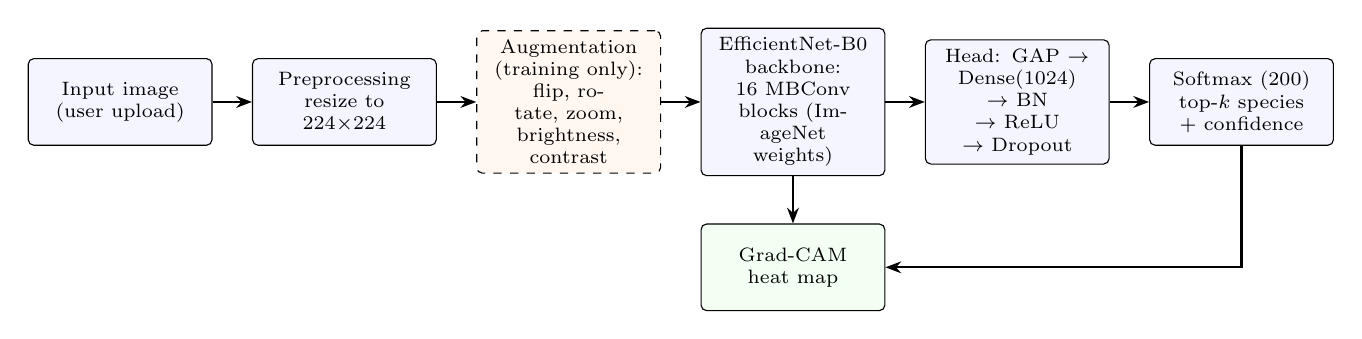
\begin{tikzpicture}[
  node distance=5mm,
  box/.style={draw, rounded corners=2pt, align=center, font=\scriptsize,
              minimum height=11mm, text width=21mm, fill=blue!4},
  opt/.style={box, dashed, fill=orange!6},
  arr/.style={-{Stealth[length=2mm]}, thick}]
\node[box] (in) {Input image\\(user upload)};
\node[box, right=of in] (pre) {Preprocessing\\resize to\\$224{\times}224$};
\node[opt, right=of pre] (aug) {Augmentation\\(training only):\\flip, rotate, zoom,\\brightness, contrast};
\node[box, right=of aug] (bb) {EfficientNet-B0\\backbone: 16 MBConv\\blocks (ImageNet\\weights)};
\node[box, right=of bb] (head) {Head: GAP $\rightarrow$\\Dense(1024) $\rightarrow$ BN\\$\rightarrow$ ReLU $\rightarrow$ Dropout};
\node[box, right=of head] (out) {Softmax (200)\\top-$k$ species\\+ confidence};
\node[box, below=6mm of bb, fill=green!5] (cam) {Grad-CAM\\heat map};
\draw[arr] (in) -- (pre); \draw[arr] (pre) -- (aug); \draw[arr] (aug) -- (bb);
\draw[arr] (bb) -- (head); \draw[arr] (head) -- (out);
\draw[arr] (bb.south) -- (cam.north);
\draw[arr] (out.south) |- (cam.east);
\end{tikzpicture}
\caption{Overview of the proposed bird species identification system. The dashed
stage is applied only during training. Grad-CAM combines the gradients of the
predicted class with the last convolutional feature maps to explain each prediction.}
\label{fig:pipeline}
\end{figure*}

\subsection{System Overview}
Fig.~\ref{fig:pipeline} summarises the system. A user supplies a photograph of a
bird. The image is resized, and during training it is also randomly augmented.
The EfficientNet-B0 backbone extracts convolutional feature maps, which the
classification head converts into a probability distribution over the 200
species. The system returns the most likely species with their confidence
scores, and a Grad-CAM heat map that shows which regions of the image supported
the prediction.

\subsection{Dataset}
We use the Caltech-UCSD Birds-200-2011 (CUB-200-2011) dataset~\cite{wah2011},
which contains 11,788 images of 200 North American bird species. We use the
official split of 5,994 training and 5,794 test images, which makes our results
directly comparable with published work. From the official training images we
hold out a stratified 10\% (the same fraction of every species) as a validation
set, which is used for early stopping, learning-rate scheduling and model
selection. This gives \NTrain{} training, \NVal{} validation and \NTest{} test
images. The test set is used only for the final evaluation. Only image-level species labels are
used; the bounding boxes and part annotations supplied with the dataset are not
used for training or testing.


\subsection{Preprocessing and Data Augmentation}\label{sec:aug}
All images are resized to $224\times224$ pixels, the input resolution of all three
backbones, and normalised exactly as during each backbone's ImageNet pretraining
(for EfficientNet-B0 this normalisation is built into the network). To improve
generalisation and reduce the effect of variations in viewpoint, scale and
lighting, the following random transformations are applied to every training
image (and never to validation or test images)~\cite{shorten2019}:
\begin{itemize}
\item horizontal flipping, since birds face left and right equally often;
\item rotation within $\pm15^\circ$, to simulate natural variation in orientation;
\item zooming by up to $\pm20\%$, to provide robustness to distance and cropping;
\item brightness and contrast changes of up to $\pm20\%$, to cope with varying illumination.
\end{itemize}

\subsection{Model Architecture}
The backbone of the proposed system is EfficientNet-B0~\cite{tan2019} pretrained
on ImageNet, with its original classification layer removed. It begins with a
$3\times3$ convolution followed by 16 mobile inverted bottleneck (MBConv)
blocks~\cite{sandler2018} arranged in seven stages, and ends with a $1\times1$
convolution to 1280 channels. Each MBConv block expands its input with a
$1\times1$ convolution, applies a depthwise $3\times3$ or $5\times5$ convolution,
recalibrates the channels with a squeeze-and-excitation unit~\cite{hu2018}, and
projects back with a $1\times1$ convolution, with a residual connection when the
input and output shapes match. All convolutions are followed by batch
normalisation and, except for the projections, by the Swish
activation~\cite{ramachandran2017}. For a $224\times224$ input the backbone
produces a $7\times7\times1280$ feature map.

The classification head consists of:
\begin{itemize}
\item global average pooling (GAP), which reduces the feature map to a
1280-dimensional vector. Flattening would instead produce a 62,720-dimensional
vector and over 64 million weights in the next layer; GAP keeps the head small
and less prone to overfitting;
\item a fully connected layer with 1024 units, followed by batch
normalisation~\cite{ioffe2015} and ReLU activation;
\item dropout~\cite{srivastava2014} with rate 0.5;
\item a fully connected output layer with 200 units and softmax activation.
\end{itemize}
Table~\ref{tab:arch} lists the parameters of each part; the complete model has
\EffNetParams{} parameters. The VGG16~\cite{simonyan2015} and
ResNet50~\cite{he2016} models used for comparison have exactly the same head on
top of their own backbones, whose final feature maps have 512 and 2048 channels.

\begin{table}[!htb]
\centering
\caption{Architecture of the proposed model}
\label{tab:arch}
\adjustbox{max width=\columnwidth}{%
\begin{tabular}{@{}llr@{}}
\toprule
Layer(s) & Output shape & Parameters \\
\midrule
EfficientNet-B0 backbone (stem conv,  & $7\times7\times1280$ & \ArchBackbone \\
\quad 16 MBConv blocks, $1\times1$ conv) & & \\
Global average pooling              & 1280                  & 0 \\
Dense + batch norm.\ + ReLU          & 1024                  & \ArchFc \\
Dropout (0.5)                       & 1024                  & 0 \\
Dense + softmax                     & 200                   & \ArchOut \\
\midrule
Total                               &                       & \ArchTotal \\
\bottomrule
\end{tabular}}
\end{table}

\subsection{Two-Stage Training}
Training proceeds in two stages, following the observation that pretrained
low-level features transfer well while high-level features benefit from
adaptation~\cite{yosinski2014}:
\begin{enumerate}
\item \emph{Stage 1 (frozen backbone).} All backbone weights are frozen and only
the head (\MainFrozenTrainable{} trainable parameters for EfficientNet-B0) is
trained with the Adam optimiser~\cite{kingma2015} at a learning rate of $10^{-3}$.
\item \emph{Stage 2 (fine-tuning).} The top of the backbone is unfrozen and the
whole network is trained further at a learning rate of $10^{-4}$. For
EfficientNet-B0 this comprises stages 5--7 and the final $1\times1$ convolution;
for VGG16, convolutional blocks 4 and 5; and for ResNet50, stages conv4 and conv5.
Batch-normalisation layers inside the backbone remain frozen, so that their
ImageNet statistics are not disturbed by the small mini-batches.
\end{enumerate}
In both stages the training is stopped when the validation loss has not improved
for 5 epochs, and the weights from the epoch with the lowest validation loss are
restored. The learning rate is halved when the validation loss stops improving
for 2 epochs. Table~\ref{tab:hyper} summarises these settings. For
EfficientNet-B0, stage~1 lasted \EpochsStageOne{} epochs and
stage~2 lasted \EpochsStageTwo{} epochs. The stage-2 setting was chosen on the
validation set: in a preliminary experiment with VGG16, fine-tuning only the last
block at $10^{-5}$ gave a validation accuracy of 62.5\%, compared with 67.8\% for
the setting above, which we then used for all models.

\begin{table}[!htb]
\centering
\caption{Training hyperparameters (identical for all backbones)}
\label{tab:hyper}
\adjustbox{max width=\columnwidth}{%
\begin{tabular}{@{}lll@{}}
\toprule
Hyperparameter & Stage 1 & Stage 2 \\
\midrule
Trainable layers     & head only        & head + top of backbone \\
Optimiser            & Adam             & Adam \\
Initial learning rate& $10^{-3}$        & $10^{-4}$ \\
Batch size           & 32               & 32 \\
Maximum epochs       & 30               & 30 \\
Early stopping       & patience 5       & patience 5 \\
LR reduction         & $\times0.5$, patience 2 & $\times0.5$, patience 2 \\
Loss                 & \multicolumn{2}{l}{categorical cross-entropy} \\
\bottomrule
\end{tabular}}
\end{table}

\subsection{Backbone Selection}
VGG16, ResNet50 and EfficientNet-B0 are trained with identical data,
preprocessing, augmentation, head and two-stage schedule. The backbone used in
the system is the one with the highest top-1 accuracy on the validation set, so
that the test set plays no part in the choice. The validation accuracies are
\VggVal\% for VGG16, \ResNetVal\% for ResNet50 and \EffNetVal\% for
EfficientNet-B0, which is therefore selected.

\subsection{Mathematical Formulation}
A standard convolutional layer computes feature maps
\begin{equation}
Z = (X * W) + b,
\end{equation}
where $X$ is the input, $W$ a set of learnable kernels and $b$ the bias. The
depthwise convolution inside an MBConv block applies one kernel $K_c$ to each
input channel separately, $Z_c = X_c * K_c$, and is followed by a pointwise
$1\times1$ convolution that mixes the channels; this factorisation needs far
fewer parameters and operations than a full convolution~\cite{sandler2018}. The
squeeze-and-excitation unit~\cite{hu2018} rescales each channel $c$ by a learned
gate,
\begin{equation}
s = \sigma\big(W_2\,\delta(W_1\,\mathrm{GAP}(X))\big),\qquad \tilde{X}_c = s_c X_c,
\end{equation}
where $\sigma$ is the sigmoid and $\delta$ the activation function. The backbone
uses the Swish activation $f(x) = x\,\sigma(x)$~\cite{ramachandran2017}, and the
head uses ReLU, $f(x)=\max(0,x)$. Batch normalisation standardises each
activation using the mini-batch mean $\mu_B$ and variance $\sigma_B^2$ and then
rescales it,
\begin{equation}
\hat{x} = \gamma\,\frac{x-\mu_B}{\sqrt{\sigma_B^2+\epsilon}} + \beta,
\end{equation}
where $\gamma$ and $\beta$ are learned. The softmax layer converts the output
logits $z_i$ into class probabilities over the $K=200$ species,
\begin{equation}
\hat{y}_i = \frac{e^{z_i}}{\sum_{j=1}^{K} e^{z_j}},
\end{equation}
and the model is trained by minimising the categorical cross-entropy between
the one-hot label $y$ and the prediction $\hat{y}$,
\begin{equation}
L = -\sum_{i=1}^{K} y_i \log \hat{y}_i .
\end{equation}
The parameters are updated with Adam~\cite{kingma2015}, which combines momentum
with per-parameter adaptive learning rates.

\subsection{Evaluation Metrics}
For a multi-class problem, the confusion-matrix counts are defined per species.
For species $k$: a \emph{true positive} ($TP_k$) is a test image of species $k$
predicted as $k$; a \emph{false positive} ($FP_k$) is an image of another species
predicted as $k$; a \emph{false negative} ($FN_k$) is an image of species $k$
predicted as another species; and a \emph{true negative} ($TN_k$) is an image of
another species not predicted as $k$. From these,
\begin{equation}
P_k = \frac{TP_k}{TP_k+FP_k},\qquad R_k = \frac{TP_k}{TP_k+FN_k},
\end{equation}
\begin{equation}
F1_k = 2\,\frac{P_k\,R_k}{P_k+R_k}.
\end{equation}
Macro-averaged precision, recall and F1-score are the means of $P_k$, $R_k$ and
$F1_k$ over all 200 species, so every species counts equally. Top-1 accuracy is
the fraction of test images whose most probable predicted species is correct,
\begin{equation}
\text{Acc} = \frac{1}{N}\sum_{n=1}^{N}\mathbb{1}\left[\arg\max_k \hat{y}_{n,k} = c_n\right],
\end{equation}
and top-5 accuracy counts a prediction as correct if the true species $c_n$ is among
the five most probable. We also report the macro-averaged one-vs-rest area
under the ROC curve (AUC) and the mean average precision (mAP), which evaluate the
ranking of the predicted probabilities rather than only the top prediction.

\subsection{Grad-CAM Visual Explanations}
To explain a prediction for class $c$, Grad-CAM~\cite{selvaraju2017} weights each
feature map $A^m$ of the last convolutional layer of the backbone (the
$7\times7\times1280$ output of the final $1\times1$ convolution of
EfficientNet-B0) by the spatially averaged gradient of the class score $y^c$,
\begin{equation}
\alpha_m^c = \frac{1}{Z}\sum_{i}\sum_{j}\frac{\partial y^c}{\partial A^m_{ij}},
\qquad
L^c = \mathrm{ReLU}\Big(\sum_m \alpha_m^c A^m\Big),
\end{equation}
and the map $L^c$ is upsampled to the image size and overlaid on the input.

% ===========================================================================
\section{Results and Discussion}\label{sec:results}
% ===========================================================================
\subsection{Experimental Setup}
All models were implemented in TensorFlow/Keras~\cite{abadi2016} and trained on a
single \TrainDevice{} GPU with mixed-precision arithmetic. All reported numbers are
computed on the \NTest{} official test images and all 200 species. Inference time
is the median time to classify a single image (batch size 1) on a
\LatencyDevice, with all models timed in the same session, and model size is the
storage needed for the weights in 32-bit floating point.

\begin{table*}[!t]
\centering
\caption{Results on CUB-200-2011 (200 species). Val.\ = top-1 accuracy on the validation set used for model selection; all other columns are on the 5,794 test images. ``Frozen'' is the top-1 accuracy after stage 1 only. P, R and F1 are macro-averaged. Latency is measured for one image at a time on a \LatencyDevice.}
\label{tab:main}
\adjustbox{max width=\textwidth}{%
\begin{tabular}{@{}lccccccccccc@{}}
\toprule
Model & Val.\ (\%) & Frozen (\%) & Top-1 (\%) & Top-5 (\%) & P (\%) & R (\%) & F1 (\%) & AUC & Params & Size (MB) & Latency (ms) \\
\midrule
VGG16~\cite{simonyan2015}  & \VggVal & \VggTopOneFrozen & \VggTopOne & \VggTopFive & \VggMacroP & \VggMacroR & \VggMacroF & \VggAUC & \VggParams & \VggSizeMB & \VggLatency \\
ResNet50~\cite{he2016}     & \ResNetVal & \ResNetTopOneFrozen & \ResNetTopOne & \ResNetTopFive & \ResNetMacroP & \ResNetMacroR & \ResNetMacroF & \ResNetAUC & \ResNetParams & \ResNetSizeMB & \ResNetLatency \\
\textbf{EfficientNet-B0~\cite{tan2019} (proposed)} & \textbf{\EffNetVal} & \textbf{\EffNetTopOneFrozen} & \textbf{\EffNetTopOne} & \textbf{\EffNetTopFive} & \textbf{\EffNetMacroP} & \textbf{\EffNetMacroR} & \textbf{\EffNetMacroF} & \textbf{\EffNetAUC} & \EffNetParams & \EffNetSizeMB & \EffNetLatency \\
\midrule
\multicolumn{12}{@{}l}{\emph{Ablation: trained without data augmentation}} \\
VGG16                      & \VggNoAugVal & \VggNoAugTopOneFrozen & \VggNoAugTopOne & \VggNoAugTopFive & \VggNoAugMacroP & \VggNoAugMacroR & \VggNoAugMacroF & \VggNoAugAUC & \VggNoAugParams & \VggNoAugSizeMB & \VggNoAugLatency \\
\EffNetNoAugRow
\bottomrule
\end{tabular}}
\end{table*}

\subsection{Backbone Comparison}
Table~\ref{tab:main} reports the validation and test performance of the three
backbones and of the ablated variants. The proposed EfficientNet-B0 system reaches
a top-1 accuracy of \EffNetTopOne\%, a top-5 accuracy of \EffNetTopFive\%, a macro
precision of \EffNetMacroP\%, a macro recall of \EffNetMacroR\% and a macro
F1-score of \EffNetMacroF\%, with a macro AUC of \EffNetAUC. It outperforms
ResNet50 (\ResNetTopOne\% top-1) and VGG16 (\VggTopOne\%) on every accuracy metric
in the table, although it has the fewest parameters of the three (\EffNetParams{} against \ResNetParams{}
and \VggParams). It is also by far the cheapest in arithmetic: EfficientNet-B0
needs 0.39 billion floating-point operations per image, compared with 4.1 billion
for ResNet50~\cite{tan2019}. On the CPU it classifies an image in \EffNetLatency{}~ms,
more than three times faster than ResNet50 (\ResNetLatency{}~ms) and about nine
times faster than VGG16 (\VggLatency{}~ms). Even with its backbone frozen,
EfficientNet-B0 (\EffNetTopOneFrozen\%) is more accurate than the fine-tuned VGG16.
The ranking on the test set agrees with the ranking on the validation set used for
model selection.

\subsection{Effect of Fine-Tuning and Data Augmentation}
\emph{Fine-tuning.} The ``Frozen'' column of Table~\ref{tab:main} shows the
accuracy reached with the backbone frozen. Fine-tuning the top of the backbone
improves the top-1 accuracy of every model: by \FineTuneGain{} percentage points
for EfficientNet-B0, \FineTuneGainResNet{} for ResNet50 and \FineTuneGainVgg{} for
VGG16. Adapting the high-level ImageNet features to birds is therefore essential
in this fine-grained setting. The gain is largest for VGG16 and ResNet50, whose
frozen features are weaker than those of EfficientNet-B0.

\emph{Data augmentation.} Contrary to our expectation, the augmentation
described in Section~\ref{sec:aug} did not improve accuracy. For VGG16, the
model trained without augmentation reaches the same top-1 accuracy
(\VggNoAugTopOne\% against \VggTopOne\%), with a top-5 accuracy only 1.3
points lower. For EfficientNet-B0, the model trained without
augmentation reaches \EffNetNoAugTopOne\% top-1 accuracy on the test set, 1.7
points more than the augmented model, although both reach the same validation
accuracy (\EffNetVal\%); the difference is already present after stage~1
(\EffNetNoAugTopOneFrozen\% against \EffNetTopOneFrozen\%). We keep the augmented
model as the proposed system because the design and the selection criterion were
fixed before testing, and the validation set, with three images per species,
cannot distinguish the two variants; we report the difference so that readers can
weigh it. One possible explanation is that, with strong pretrained features and
early stopping limiting training to a few epochs, the extra variability introduced
by rotation and zoom slows the fitting of the head more than it improves
generalisation. Augmentation designed for fine-grained recognition is left for
future work.

\begin{figure}[!htb]
\centering
\genpanel{fig_curves.pdf}{0 0 250 0}\\[2pt]
\genpanel{fig_curves.pdf}{254 0 0 0}
\caption{Training and validation accuracy (top) and loss (bottom) of the proposed
EfficientNet-B0 model. Epochs to the left of the dashed line belong to stage~1
(frozen backbone); those to the right belong to stage~2 (fine-tuning).}
\label{fig:curves}
\end{figure}

\subsection{Training Behaviour}
Fig.~\ref{fig:curves} shows the accuracy and loss of the proposed model on the
training and validation sets over both stages; the dashed line marks the start
of fine-tuning. Training curves are computed on augmented images and with dropout
active, while validation curves are not, so the two are not directly comparable
in absolute terms. The widening gap between them, with training accuracy
approaching 100\%, shows that the model can memorise the roughly 27 training
images per species; early stopping on the validation loss limits this
overfitting.

\begin{figure}[!htb]
\centering
\genpanel{fig_roc_pr.pdf}{0 0 250 0}\\[2pt]
\genpanel{fig_roc_pr.pdf}{254 0 0 0}
\caption{Micro-averaged ROC curves (top, logarithmic false positive rate) and
precision--recall curves (bottom) on the test set.}
\label{fig:rocpr}
\end{figure}

\begin{figure*}[!t]
\centering
\genfig{fig_gradcam.png}{\textwidth}
\caption{Example outputs of the system. Top: test images with their true species.
Bottom: predicted species, confidence and Grad-CAM heat map (red = regions that
contributed most). The last two columns are misclassifications.}
\label{fig:gradcam}
\end{figure*}

\subsection{ROC and Precision--Recall Analysis}
Fig.~\ref{fig:rocpr} shows the micro-averaged ROC and precision--recall curves
of the three fine-tuned backbones and of the frozen EfficientNet-B0, obtained by
treating each of the $5{,}794\times200$ image--species pairs as a binary decision.
The proposed model reaches a macro AUC of \EffNetAUC{} and a mAP of \EffNetMAP\%.
The false positive rate is plotted on a logarithmic scale because, with 200
classes, the operating points of interest lie at very low false positive rates.

\subsection{Visual Explanations}
Fig.~\ref{fig:gradcam} shows randomly chosen test images with their Grad-CAM
heat maps for four correct and two incorrect predictions of the proposed model.
In all six cases the highest activations lie on the bird, mostly on the head and
upper body, rather than on the branches, water or vegetation in the background,
which indicates that the model has learned features of the birds themselves. Both
errors involve small, drably coloured songbirds with similar silhouettes: an
Olive-sided Flycatcher predicted as a White-eyed Vireo and a Bank Swallow
predicted as a Western Wood-Pewee. The first of these was predicted with a
confidence of only 49\%, which illustrates how the confidence score can flag
uncertain identifications for review by a human expert.

\begin{table}[!htb]
\centering
\caption{Top-1 accuracy reported in the literature on CUB-200-2011 (no bounding boxes at test time)}
\label{tab:sota}
\adjustbox{max width=\columnwidth}{%
\begin{tabular}{@{}llr@{}}
\toprule
Method & Backbone & Top-1 (\%) \\
\midrule
Part-based R-CNN~\cite{zhang2014}  & AlexNet-based R-CNN & 73.9 \\
Bilinear CNN~\cite{lin2015}       & VGG-M + VGG16       & 84.1 \\
RA-CNN~\cite{fu2017}              & VGG19               & 85.3 \\
TransFG~\cite{he2022}             & ViT-B/16            & 91.7 \\
\midrule
Proposed system                    & EfficientNet-B0     & \EffNetTopOne \\
\bottomrule
\end{tabular}}
\end{table}

\subsection{Comparison with the Literature}
To place these results in context, Table~\ref{tab:sota} lists accuracies reported
in the literature for methods designed specifically for fine-grained recognition.
These methods use part localisation, attention or transformer backbones and, in
several cases, higher input resolutions, so the comparison is indicative rather
than controlled. They show the accuracy that specialised architectures can reach,
whereas the proposed system uses a compact standard backbone at $224\times224$
pixels and a simple training procedure that is easy to reproduce and deploy.

\subsection{Per-Species Analysis}
Aggregate accuracy hides differences between species. Fig.~\ref{fig:f1hist} shows
the distribution of per-species F1-scores of the proposed model. They range from
\MinClassF\% to \MaxClassF\% with a median of \MedianClassF\%, and
\NClassesBelowHalf{} of the 200 species have an F1-score below 50\%.
Table~\ref{tab:bestworst} lists the five best- and worst-recognised species. The
best-recognised species, such as the Parakeet Auklet, which is classified without
a single error, and the White-breasted Kingfisher, have distinctive shapes or
colour patterns. The worst-recognised species belong to groups that are notoriously
difficult even for experienced birders: crows, terns, large gulls and the drab
Western Wood-Pewee. Table~\ref{tab:confused} confirms this: all six of the most
frequent confusions are between closely related look-alike species, namely Common
and Arctic Terns, Caspian and Elegant Terns (in both directions), Acadian and
Least Flycatchers, and American Crow and Common Raven (in both directions). The
model's errors are therefore concentrated where the visual differences are
genuinely subtle, rather than spread at random.

Fig.~\ref{fig:cm} shows the full $200\times200$ confusion matrix, normalised by
row. Because CUB-200-2011 numbers related species consecutively (for example,
the gulls, terns, sparrows and warblers each form contiguous blocks), confusions
between closely related, visually similar species appear as off-diagonal entries
close to the diagonal, whereas confusions between unrelated species appear far
from it.

\begin{figure}[!htb]
\centering
\genfig{fig_f1hist.pdf}{\columnwidth}
\caption{Distribution of per-species F1-scores of the proposed model on the test set.}
\label{fig:f1hist}
\end{figure}

\begin{figure}[!htb]
\centering
\genfig{fig_confusion.png}{0.95\columnwidth}
\caption{Row-normalised confusion matrix of the proposed model over all 200 species
(class indices follow the dataset's taxonomic ordering).}
\label{fig:cm}
\end{figure}

\begin{table}[!htb]
\centering
\caption{Best- and worst-recognised species (proposed model, test set; $n$ = number of test images)}
\label{tab:bestworst}
\adjustbox{max width=\columnwidth}{\gentab{table_bestworst.tex}}
\end{table}

\begin{table}[!htb]
\centering
\caption{Most frequently confused species pairs (proposed model, test set)}
\label{tab:confused}
\adjustbox{max width=\columnwidth}{\gentab{table_confused.tex}}
\end{table}

\subsection{Discussion and Limitations}
The results show that, under an identical transfer-learning protocol, the choice
of backbone matters: the compact EfficientNet-B0 is the most accurate, the
smallest and the fastest of the three networks, which makes it well suited to a
system intended for mobile or field use. Fine-tuning the top of the backbone helps
every network, whereas our data augmentation did not. The top-5 accuracy, which is relevant when the system
suggests a short list of candidate species to a human observer, is
\EffNetTopFive\%, compared with \EffNetTopOne\% for top-1. Several limitations
remain. First, CUB-200-2011 contains only North American species photographed
mostly in good conditions; performance on camera-trap or smartphone images, and on
regional species such as those of India, remains to be verified. Second, the
dataset provides about 30 training images per species, and the training curves
show clear overfitting despite augmentation, dropout and early stopping. Third, the
validation set holds only three images per species, which is too few to separate
closely matched variants such as the models with and without augmentation. Fourth,
specialised fine-grained architectures still achieve higher accuracy than our
system (Table~\ref{tab:sota}), at the cost of greater complexity. Finally, the
latencies in Table~\ref{tab:main} were measured on a \LatencyDevice; measurements on
phones would be needed to confirm the deployment advantage of EfficientNet-B0.


% ===========================================================================
\section{Conclusion and Future Work}\label{sec:conclusion}
% ===========================================================================
We presented a CNN-based bird species identification system that combines an
ImageNet-pretrained EfficientNet-B0 backbone with a regularised classification
head and two-stage transfer learning. Evaluated on the official test split of
CUB-200-2011 across all 200 species, it achieves a top-1 accuracy of
\EffNetTopOne\%, a top-5 accuracy of \EffNetTopFive\% and a macro F1-score of
\EffNetMacroF\%, outperforming VGG16 and ResNet50 trained under the same protocol
while using the fewest parameters and running fastest. Fine-tuning improved every
backbone, while the data augmentation used did not improve accuracy. The per-species
analysis shows that the remaining errors are concentrated among closely related
look-alike species, and Grad-CAM confirms that the predictions are based on the
birds rather than the background.

In future work we plan to (i)~add attention or part-localisation mechanisms to
close the gap with specialised fine-grained methods, (ii)~evaluate the system on
larger and more diverse datasets such as NABirds and iNaturalist and on regional
species, (iii)~deploy it as a mobile and web application that, in addition to the
predicted species, presents information on habitat, behaviour and conservation
status, (iv)~study augmentation strategies suited to fine-grained recognition, and
(v)~combine image-based and acoustic identification.

% keep every figure and table ahead of the references
\FloatBarrier

% ===========================================================================
\begin{thebibliography}{00}

\bibitem{krizhevsky2012} A. Krizhevsky, I. Sutskever, and G. E. Hinton,
``ImageNet classification with deep convolutional neural networks,'' in
\emph{Proc. Adv. Neural Inf. Process. Syst. (NeurIPS)}, 2012, pp. 1097--1105.

\bibitem{simonyan2015} K. Simonyan and A. Zisserman, ``Very deep convolutional
networks for large-scale image recognition,'' in \emph{Proc. Int. Conf. Learn.
Represent. (ICLR)}, 2015.

\bibitem{wah2011} C. Wah, S. Branson, P. Welinder, P. Perona, and S. Belongie,
``The Caltech-UCSD Birds-200-2011 dataset,'' California Institute of Technology,
Pasadena, CA, USA, Tech. Rep. CNS-TR-2011-001, 2011.

\bibitem{deng2009} J. Deng, W. Dong, R. Socher, L.-J. Li, K. Li, and L. Fei-Fei,
``ImageNet: A large-scale hierarchical image database,'' in \emph{Proc. IEEE Conf.
Comput. Vis. Pattern Recognit. (CVPR)}, 2009, pp. 248--255.

\bibitem{yosinski2014} J. Yosinski, J. Clune, Y. Bengio, and H. Lipson, ``How
transferable are features in deep neural networks?'' in \emph{Proc. Adv. Neural
Inf. Process. Syst. (NeurIPS)}, 2014, pp. 3320--3328.

\bibitem{dalal2005} N. Dalal and B. Triggs, ``Histograms of oriented gradients for
human detection,'' in \emph{Proc. IEEE Conf. Comput. Vis. Pattern Recognit.
(CVPR)}, 2005, pp. 886--893.

\bibitem{ojala2002} T. Ojala, M. Pietik\"ainen, and T. M\"aenp\"a\"a,
``Multiresolution gray-scale and rotation invariant texture classification with
local binary patterns,'' \emph{IEEE Trans. Pattern Anal. Mach. Intell.}, vol.~24,
no.~7, pp. 971--987, 2002.

\bibitem{cortes1995} C. Cortes and V. Vapnik, ``Support-vector networks,''
\emph{Mach. Learn.}, vol.~20, no.~3, pp. 273--297, 1995.

\bibitem{he2016} K. He, X. Zhang, S. Ren, and J. Sun, ``Deep residual learning for
image recognition,'' in \emph{Proc. IEEE Conf. Comput. Vis. Pattern Recognit.
(CVPR)}, 2016, pp. 770--778.

\bibitem{tan2019} M. Tan and Q. V. Le, ``EfficientNet: Rethinking model scaling for
convolutional neural networks,'' in \emph{Proc. Int. Conf. Mach. Learn. (ICML)},
2019, pp. 6105--6114.

\bibitem{sandler2018} M. Sandler, A. Howard, M. Zhu, A. Zhmoginov, and L.-C. Chen,
``MobileNetV2: Inverted residuals and linear bottlenecks,'' in \emph{Proc. IEEE
Conf. Comput. Vis. Pattern Recognit. (CVPR)}, 2018, pp. 4510--4520.

\bibitem{shorten2019} C. Shorten and T. M. Khoshgoftaar, ``A survey on image data
augmentation for deep learning,'' \emph{J. Big Data}, vol.~6, Art. no. 60, 2019.

\bibitem{sravanthi2025plant} P. Naga Sravanthi, S. H. Vardhan Chikkala, T. R. Tumma,
and L. V. S. Paila, ``Hybrid deep learning pipeline with CNN-based feature
embeddings and dimensionality reduction for plant disease detection,'' in
\emph{Proc. 1st IEEE Int. Conf. Data Sci. Intell. Netw. Comput. (ICDSINC)}, 2025,
pp. 735--740, doi: 10.1109/ICDSINC66221.2025.11448138.

\bibitem{sravanthi2026vgg19} P. Naga Sravanthi, R. R. Sannapureddy, C. Lakkimsetti,
N. S. Vistamsetty, and K. Chaganti, ``Visionary harvest: Integrating custom blur
layers into VGG19 for obscured edible classification,'' in \emph{Proc. 9th Int.
Conf. Comput. Methodol. Commun. (ICCMC)}, 2026, pp. 1548--1553,
doi: 10.1109/ICCMC69250.2026.11625194.

\bibitem{zhang2014} N. Zhang, J. Donahue, R. Girshick, and T. Darrell, ``Part-based
R-CNNs for fine-grained category detection,'' in \emph{Proc. Eur. Conf. Comput.
Vis. (ECCV)}, 2014, pp. 834--849.

\bibitem{lin2015} T.-Y. Lin, A. RoyChowdhury, and S. Maji, ``Bilinear CNN models for
fine-grained visual recognition,'' in \emph{Proc. IEEE Int. Conf. Comput. Vis.
(ICCV)}, 2015, pp. 1449--1457.

\bibitem{fu2017} J. Fu, H. Zheng, and T. Mei, ``Look closer to see better:
Recurrent attention convolutional neural network for fine-grained image
recognition,'' in \emph{Proc. IEEE Conf. Comput. Vis. Pattern Recognit. (CVPR)},
2017, pp. 4438--4446.

\bibitem{he2022} J. He, J.-N. Chen, S. Liu, A. Kortylewski, C. Yang, Y. Bai, and
C. Wang, ``TransFG: A transformer architecture for fine-grained recognition,'' in
\emph{Proc. AAAI Conf. Artif. Intell.}, vol.~36, no.~1, 2022, pp. 852--860.

\bibitem{vanhorn2015} G. Van Horn, S. Branson, R. Farrell, S. Haber, J. Barry,
P. Ipeirotis, P. Perona, and S. Belongie, ``Building a bird recognition app and
large scale dataset with citizen scientists: The fine print in fine-grained
dataset collection,'' in \emph{Proc. IEEE Conf. Comput. Vis. Pattern Recognit.
(CVPR)}, 2015, pp. 595--604.

\bibitem{vanhorn2018} G. Van Horn, O. Mac Aodha, Y. Song, Y. Cui, C. Sun, A. Shepard,
H. Adam, P. Perona, and S. Belongie, ``The iNaturalist species classification and
detection dataset,'' in \emph{Proc. IEEE Conf. Comput. Vis. Pattern Recognit.
(CVPR)}, 2018, pp. 8769--8778.

\bibitem{kahl2021} S. Kahl, C. M. Wood, M. Eibl, and H. Klinck, ``BirdNET: A deep
learning solution for avian diversity monitoring,'' \emph{Ecol. Inform.}, vol.~61,
Art. no. 101236, 2021.

\bibitem{gomez2022} J. G\'omez-G\'omez, E. Vida\~na-Vila, and X. Sevillano,
``Western Mediterranean wetlands bird species classification: Evaluating
small-footprint deep learning approaches on a new annotated dataset,''
arXiv:2207.05393, 2022.

\bibitem{sastry2024} S. Sastry, S. Khanal, A. Dhakal, D. Huang, and N. Jacobs,
``BirdSAT: Cross-view contrastive masked autoencoders for bird species
classification and mapping,'' in \emph{Proc. IEEE/CVF Winter Conf. Appl. Comput.
Vis. (WACV)}, 2024, pp. 7136--7145.

\bibitem{puppala2025plastic} N. S. Puppala, P. L. Sai, T. M. R. Shankar,
K. G. V. Bharadwaja \emph{et al.}, ``Detecting marine plastic waste using aerial and
satellite images---A multimodal fusion approach,'' in \emph{Proc. 1st IEEE Int.
Conf. Data Sci. Intell. Netw. Comput. (ICDSINC)}, 2025, pp. 42--47,
doi: 10.1109/ICDSINC66221.2025.11448230.

\bibitem{selvaraju2017} R. R. Selvaraju, M. Cogswell, A. Das, R. Vedantam,
D. Parikh, and D. Batra, ``Grad-CAM: Visual explanations from deep networks via
gradient-based localization,'' in \emph{Proc. IEEE Int. Conf. Comput. Vis.
(ICCV)}, 2017, pp. 618--626.

\bibitem{ribeiro2016} M. T. Ribeiro, S. Singh, and C. Guestrin, ```Why should I
trust you?': Explaining the predictions of any classifier,'' in \emph{Proc. ACM
SIGKDD Int. Conf. Knowl. Discov. Data Min. (KDD)}, 2016, pp. 1135--1144.

\bibitem{lundberg2017} S. M. Lundberg and S.-I. Lee, ``A unified approach to
interpreting model predictions,'' in \emph{Proc. Adv. Neural Inf. Process. Syst.
(NeurIPS)}, 2017, pp. 4765--4774.

\bibitem{kumar2024} S. V. S. Kumar and H. K. Kondaveeti, ``Towards transparency in
AI: Explainable bird species image classification for ecological research,''
\emph{Ecol. Indic.}, vol.~169, Art. no. 112886, 2024,
doi: 10.1016/j.ecolind.2024.112886.

\bibitem{hu2018} J. Hu, L. Shen, and G. Sun, ``Squeeze-and-excitation networks,''
in \emph{Proc. IEEE Conf. Comput. Vis. Pattern Recognit. (CVPR)}, 2018,
pp. 7132--7141.

\bibitem{ramachandran2017} P. Ramachandran, B. Zoph, and Q. V. Le, ``Searching for
activation functions,'' arXiv:1710.05941, 2017.

\bibitem{ioffe2015} S. Ioffe and C. Szegedy, ``Batch normalization: Accelerating
deep network training by reducing internal covariate shift,'' in \emph{Proc. Int.
Conf. Mach. Learn. (ICML)}, 2015, pp. 448--456.

\bibitem{srivastava2014} N. Srivastava, G. Hinton, A. Krizhevsky, I. Sutskever, and
R. Salakhutdinov, ``Dropout: A simple way to prevent neural networks from
overfitting,'' \emph{J. Mach. Learn. Res.}, vol.~15, pp. 1929--1958, 2014.

\bibitem{kingma2015} D. P. Kingma and J. Ba, ``Adam: A method for stochastic
optimization,'' in \emph{Proc. Int. Conf. Learn. Represent. (ICLR)}, 2015.

\bibitem{abadi2016} M. Abadi \emph{et al.}, ``TensorFlow: A system for large-scale
machine learning,'' in \emph{Proc. USENIX Symp. Oper. Syst. Des. Implement.
(OSDI)}, 2016, pp. 265--283.

\end{thebibliography}

\end{document}
